\newcommand{\finalFormula}{


}

\section{The Parametric Case and the Polar Case}

Suppose you want to study the $N$-Units Away Curves of a curve, but you do not have it in a simple closed $y = f(x)$ form but instead you have a parametric function $\begin{bmatrix} x(t) \\ y(t) \end{bmatrix} = \begin{bmatrix} g(t) \\ h(t) \end{bmatrix}$. Can you still find the $N$-Units Away Curves to that parametric curve in $\mathbb{R}^2$?

I had always hoped I might be able to solve for the $N$-Units Away Curves in the case, and in fact I have been able to! So long as functions $g$ and $h$ are differentiable.

Take some value of $t$. Call it $t_o$. The slope of the parametric curve at location $t = t_o$ is $ \dfrac{dy}{dx} = 
\dfrac{\dfrac{dy}{dt}}{\dfrac{dy}{dt}} = \dfrac{y'(t)}{x'(t)} = \dfrac{h'(t)}{g'(t)} $. Take note, of course, that this formula is only valid so long as $g'(t) \neq 0$. Suspend your disbelief for the moment and simply ignore those values of $t$. The final formula will address them.
    
Where before we had: $\begin{bmatrix} x \\ y \end{bmatrix} = \begin{bmatrix} t \\ f'(t) \end{bmatrix} + N \dfrac{\begin{bmatrix} -f'(t) \\ 1 \end{bmatrix}}{|\begin{bmatrix} -f'(t) \\ 1 \end{bmatrix}|}$, now replace every occurrence of $f'(t)$ with $\dfrac{h'(t)}{g'(t)}$ to get $\begin{bmatrix} x \\ y \end{bmatrix} = \begin{bmatrix} 1 \\ \dfrac{h'(t)}{g'(t)} \end{bmatrix} + N \dfrac{\begin{bmatrix} \dfrac{-h'(t)}{g'(t)} \\ 1 \end{bmatrix}}{\left| \begin{bmatrix} \dfrac{-h'(t)}{g'(t)} \\ 1 \end{bmatrix} \right|}$, when $g' \neq 0$.

However, when you graph the results, we find that like with formula 1 for the $N$-Units Away Curves, there is a problem where the graph we've so far made flips which side of the original parametric function we're on. It
switches sides inappropriately every time $g'(t)$ changes sign. Fixing this is a problem we have already previously encountered in this paper and can be rectified by multiplying by a $\dfrac{g'(t)}{|g'(t)|}$ term.

\begin{figure}[h!]
  \begin{minipage}[b]{\linewidth}
      \centering
      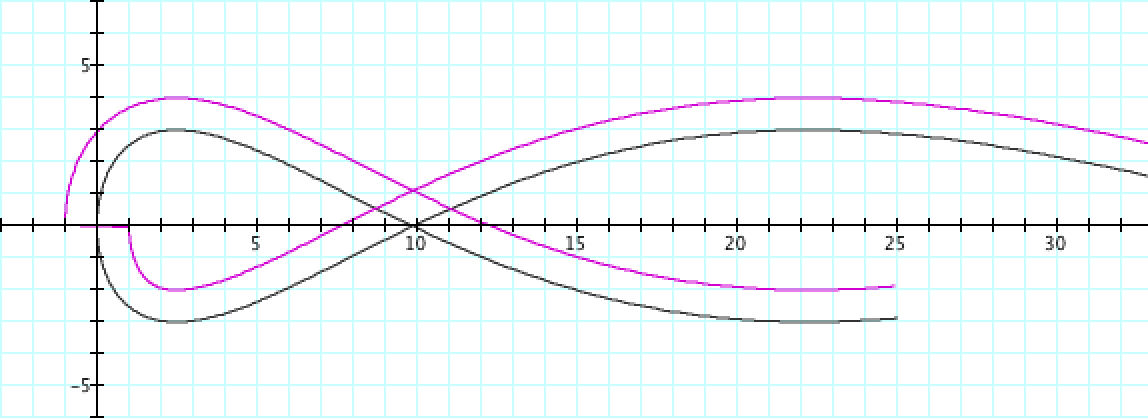
\includegraphics[width=\linewidth]{parametric-polar-img/Fig 29.png}
      \caption{}
      \label{fig:fig29}
  \end{minipage}
\end{figure}

This leaves us with one last big problem which is these discontinuities when $g'(t) = 0$. Let's see if we can invent a suitable $N$-Units Away formula that is defined even at those values.

Let's assume we have a positive value for $N$. With the original $y = f(x)$ $N$-Units Away Curve, I've described that you can think of $y = f(x)$ as being equivalent to the parametric function $\begin{bmatrix} x(t) \\ y(t) \end{bmatrix} =  \begin{bmatrix} 1 \\ f(t) \end{bmatrix}$. In this case the parametric function's $x$ term is always moving to the right, and the $N$-Units Away Curve is defined as being above the curve. It's a fairly natural extension to say that in the $\begin{bmatrix} x(t) \\ y(t) \end{bmatrix} =  \begin{bmatrix} g(t) \\ h(t) \end{bmatrix}$ case when the $x$ term is moving to the left we should define the $N$-Units Away Curve to be below the curve. In fact we just did this on the previous page with our $\dfrac{g'(t)}{|g'(t)|}$ term. When the function is going \textit{East} the $N$-Units Away Curves are placed \textit{North}. When the function is going \textit{West} the $N$-Units Away Curves are placed \textit{South}. It's always a $90^{\circ}$ turn to the left. By extension, when the function is going straight vertically \textit{North}, define that we should place the associated $N$-Units Away dot to the \textit{West}, and when the function is going straight vertically \textit{South}, define that we should place the $N$-Units Away dot to the \textit{East}. All discontinuities have thus been addressed and we arrive at the following final formula: \finalFormula.

The resultant graphs we obtain are profoundly cool looking! Check out the example of $g(t) = sin (7 \pi t)$, $h(t) = cos (5 \pi t)$ as $N$ increases from 0 up:

\begin{figure}[H] 
  \label{polar-1} 
  \centering
  \begin{minipage}[b]{0.4\linewidth}
    \centering
    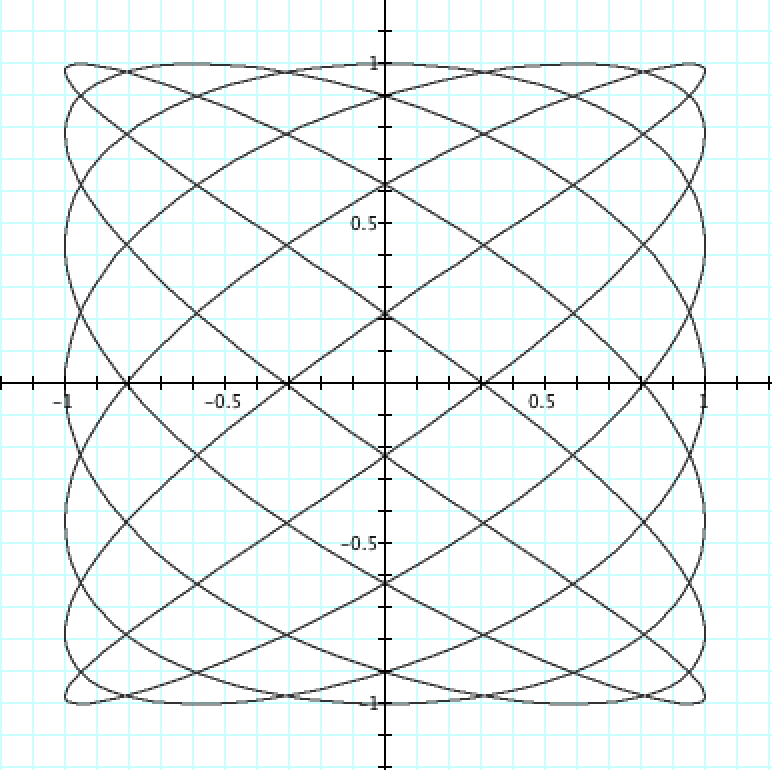
\includegraphics[width=.9\linewidth]{parametric-polar-img/Fig 30.png} 
    \caption{Caption} 
    \label{fig:fig30}
    \vspace{4ex}
  \end{minipage} % end 
  \begin{minipage}[b]{0.4\linewidth}
    \centering
    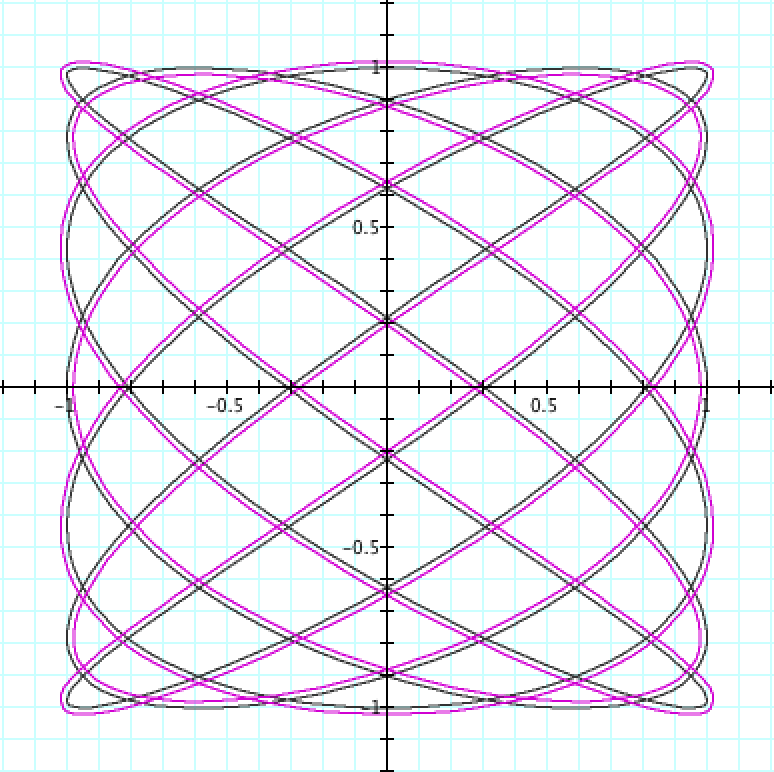
\includegraphics[width=.9\linewidth]{parametric-polar-img/Fig 31.png} 
    \caption{Caption} 
    \label{fig:fig31}
    \vspace{4ex}
  \end{minipage} % end
  \begin{minipage}[b]{0.4\linewidth}
    \centering
    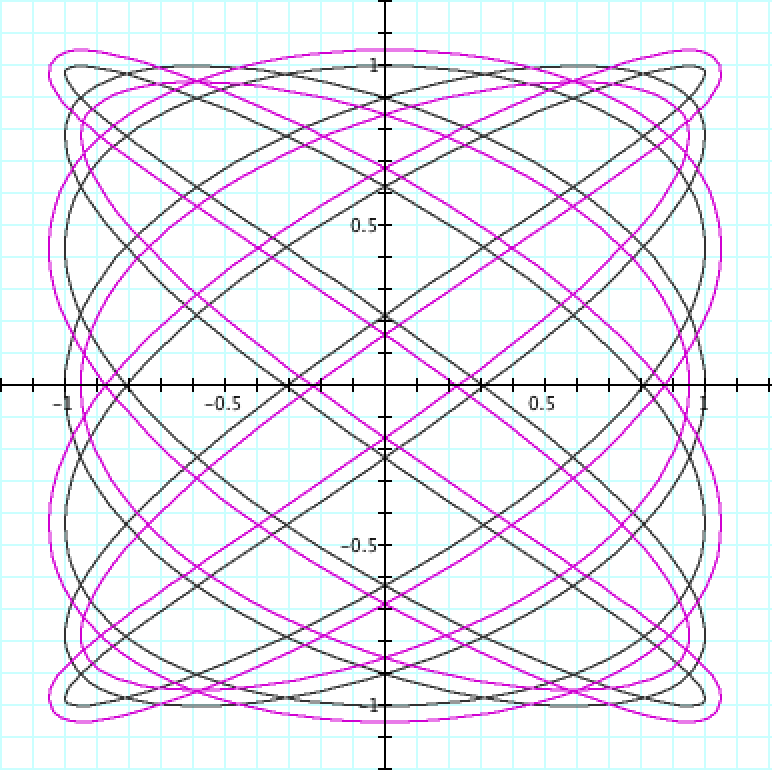
\includegraphics[width=.9\linewidth]{parametric-polar-img/Fig 32.png} 
    \caption{Caption} 
    \label{fig:fig32}
    \vspace{4ex}
  \end{minipage} % end
  \begin{minipage}[b]{0.4\linewidth}
    \centering
    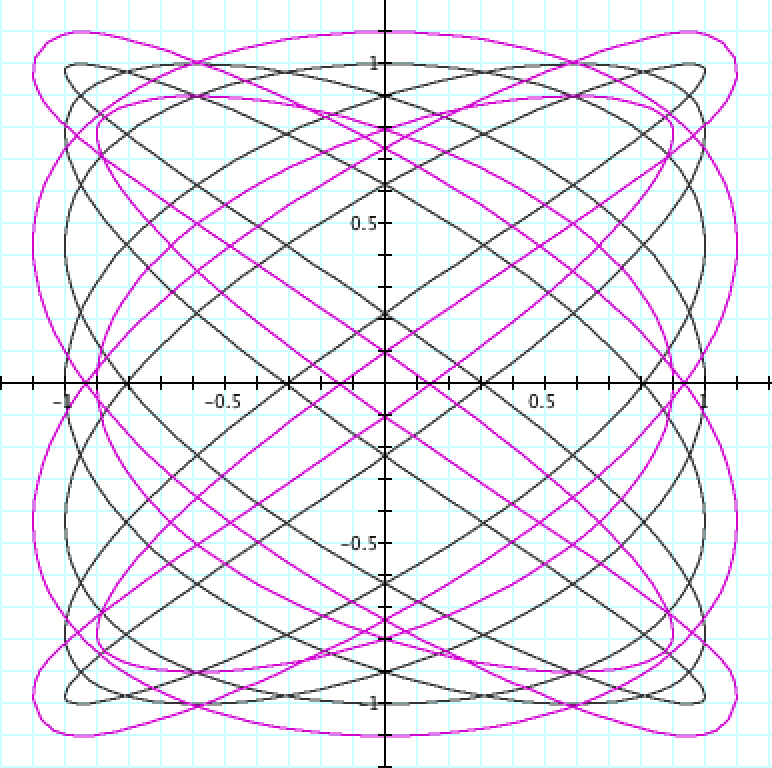
\includegraphics[width=.9\linewidth]{parametric-polar-img/Fig 33.png} 
    \caption{Caption} 
    \label{fig:fig33}
    \vspace{4ex}
  \end{minipage} % end
    \begin{minipage}[b]{0.4\linewidth}
    \centering
    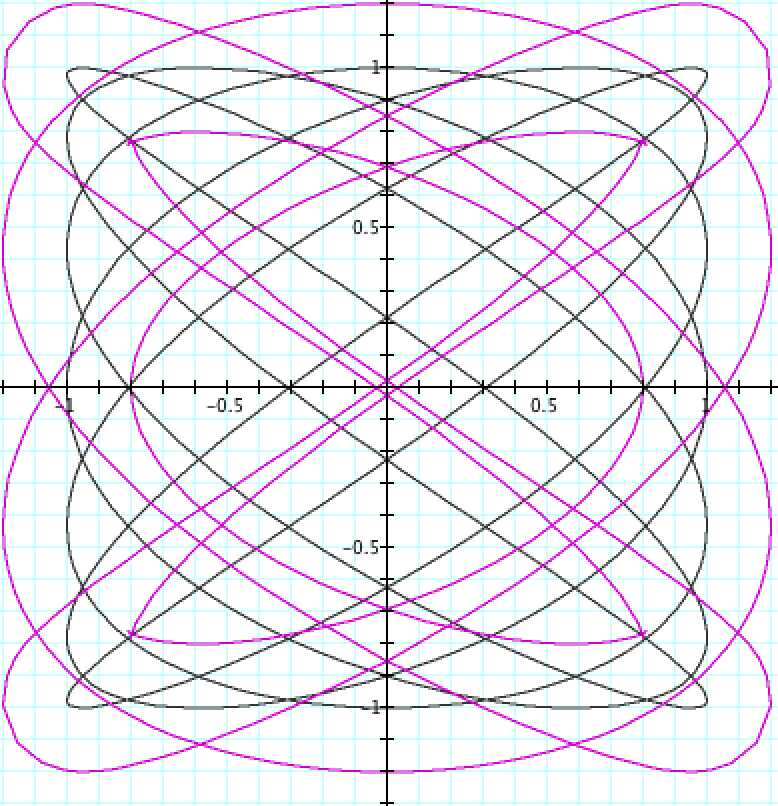
\includegraphics[width=.9\linewidth]{parametric-polar-img/Fig 34.png} 
    \caption{Caption} 
    \label{fig:fig34}
    \vspace{4ex}
  \end{minipage} % end
\end{figure}

Fabulously enough, this instantly also solves the case of Polar Functions as well! Suppose instead of a function $y = f(x)$, you have some polar function $r( \theta ) = g( \theta )$. It’s a nice little Calc 2 fact that polar functions can be represented as parametric equations by performing $r(\theta) = g(\theta) \xrightarrow{} (x(t), y(t)) = (g(t) cos(t), g(t) sin(t))$.

We can now plug this into our solution to the parametric case and obtain truly beautiful Polar $N$-Units Away Curves. Here is a gorgeous example. Let $r (\theta) = sin(\dfrac{8}{5} * \theta)$. One ends up with the following $N$-Units Away Curve:

\begin{figure}[H] 
  \label{polar-2} 
  \begin{minipage}[b]{0.5\linewidth}
    \centering
    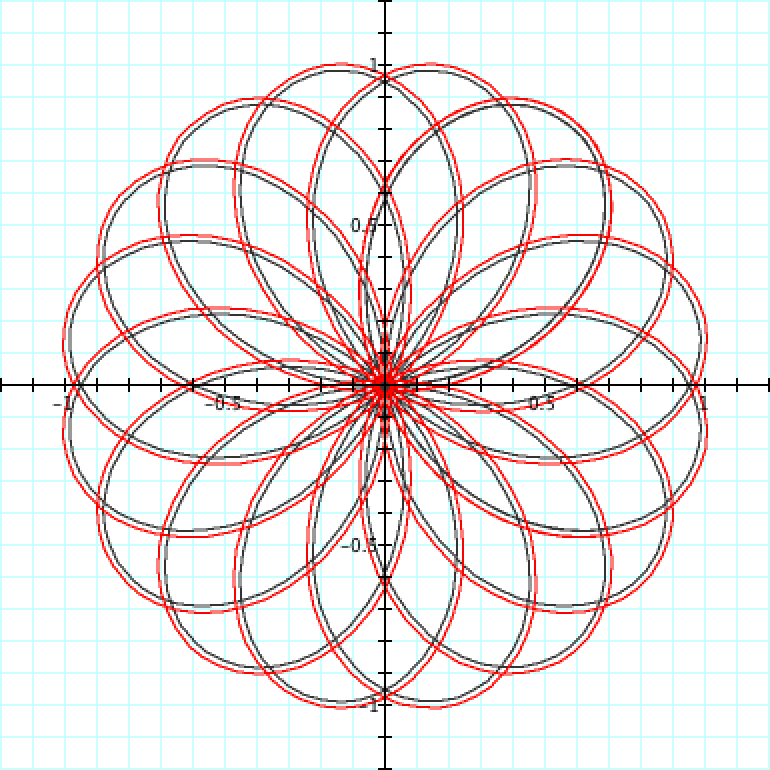
\includegraphics[width=.9\linewidth]{parametric-polar-img/Fig 35.png} 
    \caption{Caption} 
    \label{fig:fig35}
    \vspace{4ex}
  \end{minipage} % end 
  \begin{minipage}[b]{0.5\linewidth}
    \centering
    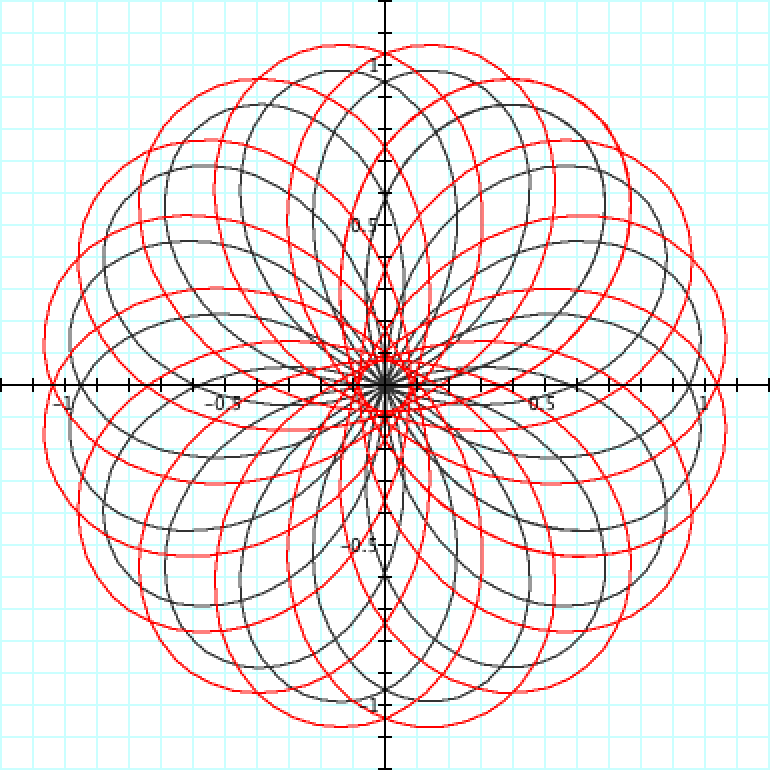
\includegraphics[width=.9\linewidth]{parametric-polar-img/Fig 36.png} 
    \caption{Caption} 
    \label{fig:fig36}
    \vspace{4ex}
  \end{minipage} % end
  \begin{minipage}[b]{0.5\linewidth}
    \centering
    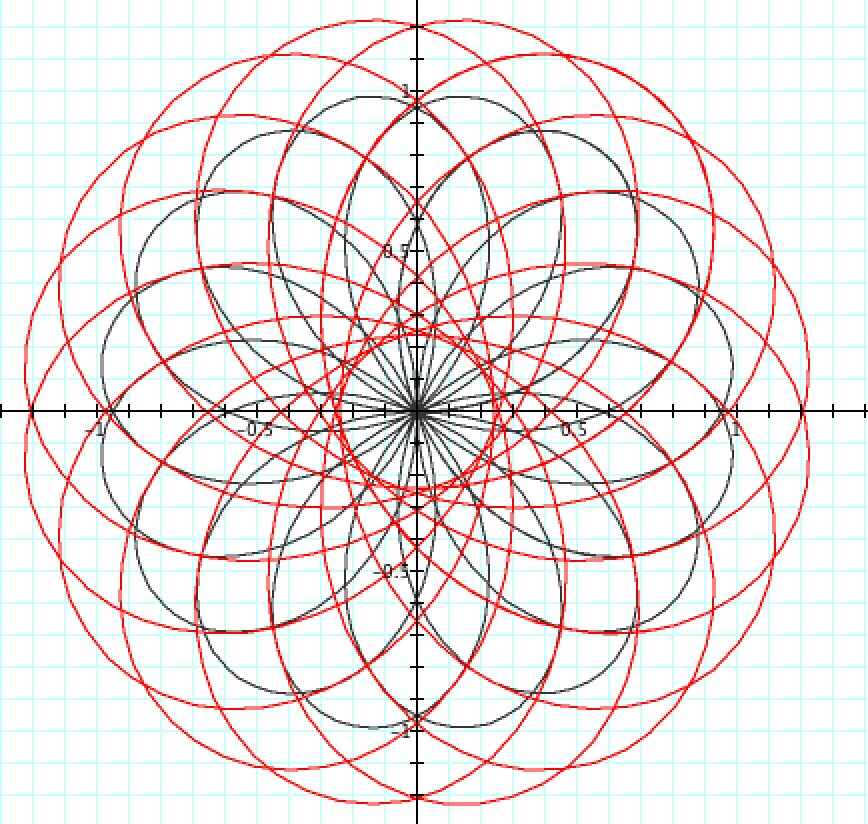
\includegraphics[width=.9\linewidth]{parametric-polar-img/Fig 37.png} 
    \caption{Caption} 
    \label{fig:fig37}
    \vspace{4ex}
  \end{minipage} % end
  \begin{minipage}[b]{0.5\linewidth}
    \centering
    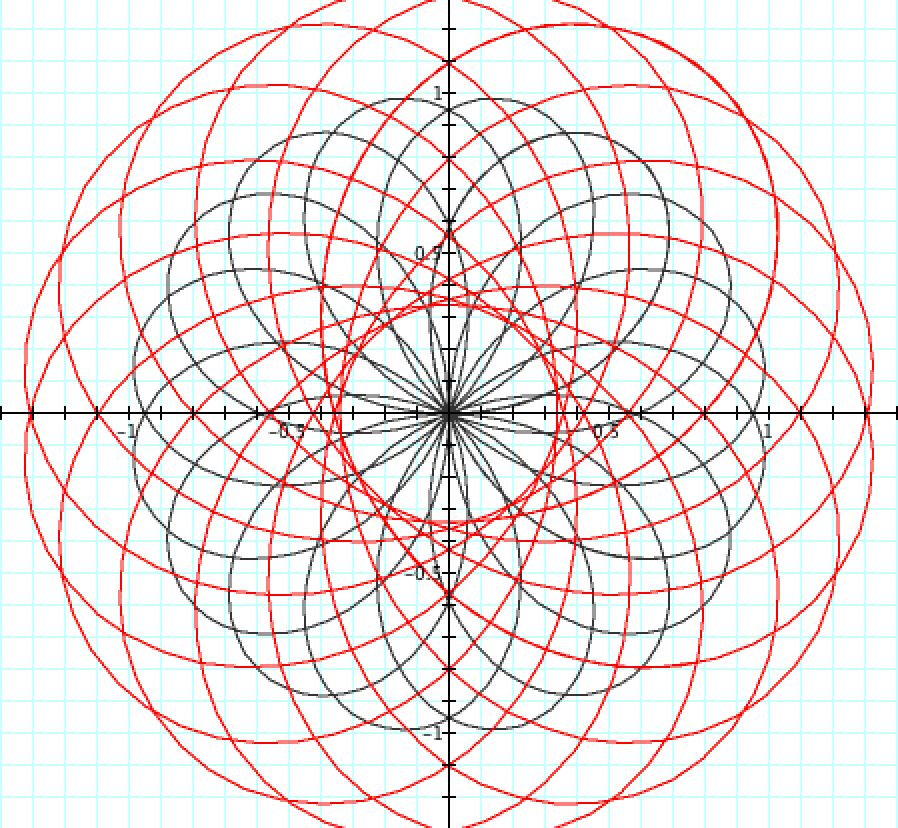
\includegraphics[width=.9\linewidth]{parametric-polar-img/Fig 38.png} 
    \caption{Caption} 
    \label{fig:fig38}
    \vspace{4ex}
  \end{minipage} % end
\end{figure}

